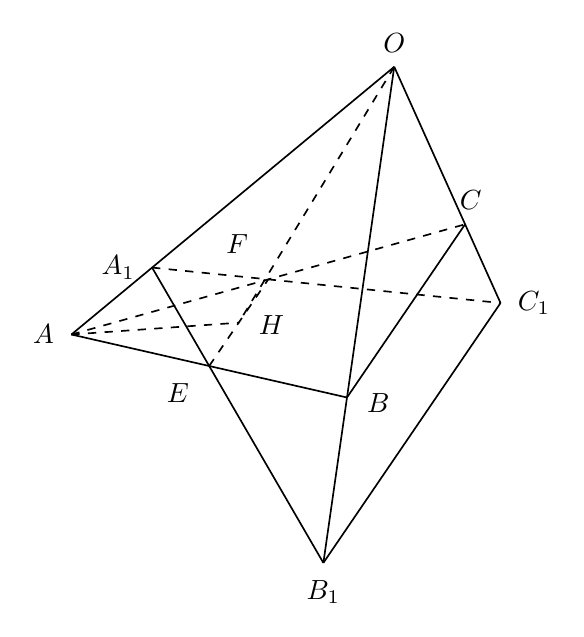
\begin{tikzpicture}[x=1cm,y=1cm,line width=.6pt,font=\normalsize,
geometry edge/.style={solid,line width=.6pt},
geometry label/.style={font=\normalsize,inner sep=2pt}]
\coordinate (O) at (2.5,3.6);
\coordinate (A) at (-1.6,0.2);
\coordinate (B) at (1.9,-0.6);
\coordinate (C) at (3.4,1.6);
\coordinate (E) at (0.15,-0.2);
\coordinate (F) at (0.9,0.9);
\coordinate (H) at (0.525,0.35);
\coordinate (A1) at (-0.575,1.05);
\coordinate (B1) at (1.6,-2.7);
\coordinate (C1) at (3.85,0.6);
% solid trihedral O-ABC
\draw[geometry edge] (O) -- (A);
\draw[geometry edge] (O) -- (B1);
\draw[geometry edge] (O) -- (C) -- (C1);
\draw[geometry edge] (A) -- (B);
\draw[geometry edge] (B) -- (C);

\draw[geometry edge] (B1) -- (C1);
\draw[geometry edge] (A1) -- (B1);
% dashed interior / cutting plane
\draw[geometry edge,dashed] (O)--(H);
\draw[geometry edge,dashed] (E)--(F);
\draw[geometry edge,dashed] (A) -- (C);
\draw[geometry edge,dashed] (A1) -- (C1);
\draw[geometry edge,dashed] (A) -- (H);
\node[geometry label,above,yshift=3pt] at (O) {$O$};
\node[geometry label,left,xshift=-4pt] at (A) {$A$};
\node[geometry label,right,xshift=5pt,yshift=-2pt] at (B) {$B$};
\node[geometry label,above,xshift=2pt,yshift=3pt] at (C) {$C$};
\node[geometry label,below left,xshift=-5pt,yshift=-4pt] at (E) {$E$};
\node[geometry label,above left,xshift=-5pt,yshift=7pt] at (F) {$F$};
\node[geometry label,right,xshift=5pt,yshift=-1pt] at (H) {$H$};
\node[geometry label,left,xshift=-4pt] at (A1) {$A_{1}$};
\node[geometry label,below,yshift=-4pt] at (B1) {$B_{1}$};
\node[geometry label,right,xshift=4pt] at (C1) {$C_{1}$};
\end{tikzpicture}
